\documentclass[border=10pt]{standalone}
\usepackage{tikz}
\usetikzlibrary{er,positioning}

\begin{document}

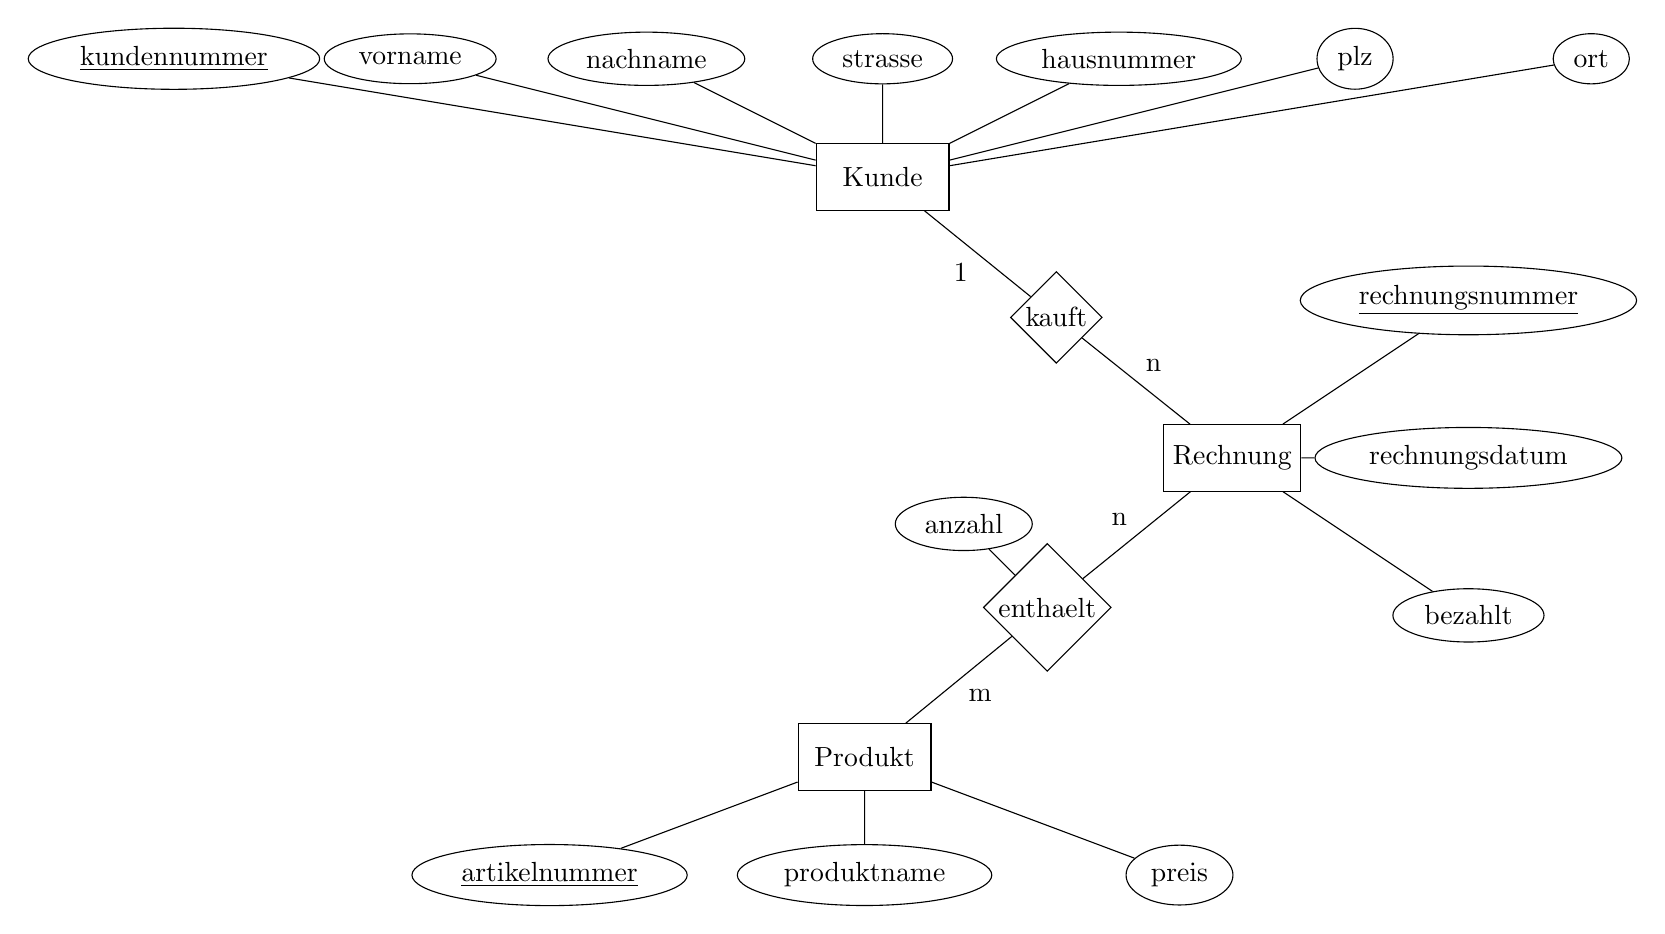
\begin{tikzpicture}[auto,node distance=1.5cm]
  \node[entity] (kunde) { Kunde }
    [grow=up,sibling distance=3cm]
    child {node[attribute] {ort}}
    child {node[attribute] {plz}}
    child {node[attribute] {hausnummer}}
    child {node[attribute] {strasse}}
    child {node[attribute] {nachname}}
    child {node[attribute] {vorname}}
    child {node[attribute] {\underline{kundennummer}}};
  \node[relationship] (kauft) [below right = of kunde] {kauft};
  \node[entity] (rechnung) [below right = of kauft]	{Rechnung}
    [grow=0,level distance=3cm, sibling distance=2cm]
    child {node[attribute] {bezahlt}}
    child {node[attribute] {rechnungsdatum}}
    child {node[attribute] {\underline{rechnungsnummer}}};
  \node[relationship] (enthaelt) [below left = of rechnung] {enthaelt}
    [grow=135,sibling distance=3cm]
    child {node[attribute] {anzahl}};
  \node[entity] (produkt) [below left = of enthaelt]	{Produkt}
    [grow=down,sibling distance=4cm]
    child {node[attribute] {\underline{artikelnummer}}}
    child {node[attribute] {produktname}}
    child {node[attribute] {preis}};
  % Draw an edge between rel1 and node1; rel1 and node2
  \path (kauft) edge node {1} (kunde)
    edge	 node {n}	(rechnung);
  \path (enthaelt) edge node {n} (rechnung)
    edge	 node {m}	(produkt);
\end{tikzpicture}
\end{document}